%!TEX root = ../thesis.tex

本章では，本研究の基盤となる要素技術について述べる．まず，物体検出について従来手法からゼロショット技術への発展を含めて詳述する．次に，セグメンテーションについて従来手法からゼロショット技術への発展を含めて詳述する．最後に，物体追跡について基本的な手法を説明する．

\section{物体検出}
物体検出は，画像内の物体の位置（以後，BBoxと呼ぶ）とカテゴリを同時に予測するコンピュータビジョンの基本的なタスクである．

\subsection{従来の物体検出とその課題}
従来の物体検出手法は，Faster R-CNN\cite{faster_rcnn}やYOLO\cite{yolo}などの深層学習モデルにより高精度な検出を実現してきた．これらの手法は，大量のラベル付きデータで学習され，固定されたカテゴリ集合に対して性能を発揮する．

しかし，従来手法には本質的な制約がある．学習時に定義されたカテゴリのみを検出可能であり，新しいカテゴリを追加するには，そのカテゴリのラベル付きデータを収集し，モデル全体を再学習する必要がある．例えば，COCOデータセット\cite{coco}で学習されたモデルは80カテゴリの物体のみを検出でき，「パイロン」や「ホワイトボード」といった新しいカテゴリには対応できない(\Fig{fig:traditional_detection})．この制約は，実世界の多様な物体を扱う上で大きな障壁となる．

\begin{figure}[H]
\centering
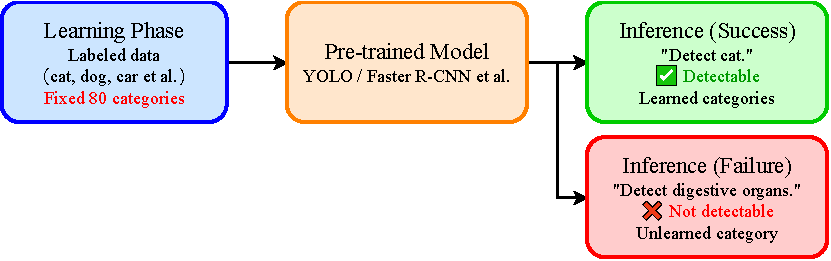
\includegraphics[width=1.0\linewidth]{images/pdf/traditional_object_detection.pdf}
\caption{Traditional object detection.}
\label{fig:traditional_detection}
\end{figure}

\newpage

\subsection{ゼロショット物体検出}
ゼロショット物体検出とは，学習時に見たことのない物体カテゴリを，テキスト記述のみで検出する技術である．従来の物体検出の制約を克服し，視覚情報と言語情報を統合することで，任意のテキストプロンプトに対応した検出を実現する．

この技術の核心は，物体の視覚的特徴と言語的記述を共通の埋め込み空間で対応付けることにある．画像はCNNまたはVision Transformerにより処理され，多スケールの特徴マップが生成される．テキストプロンプトはBERT\cite{bert}などの言語モデルによりエンコードされ，言語特徴ベクトルに変換される．視覚特徴と言語特徴は，cross-attention機構により相互作用する．言語特徴の各単語が画像特徴の各位置に対してattention重みを計算し，テキストプロンプト全体に対応する画像領域が特定される．

推論時には，ユーザーが任意のテキストプロンプトを入力でき，単一物体の記述から属性を含む記述，関係性を含む記述まで対応可能である．信頼度スコアが閾値を超える検出のみが最終結果として採用される．この柔軟性により，事前に定義されていない任意の物体カテゴリに対して対応できる(\Fig{fig:zeroshot_detection})．

\vspace{1cm}

\begin{figure}[H]
\centering
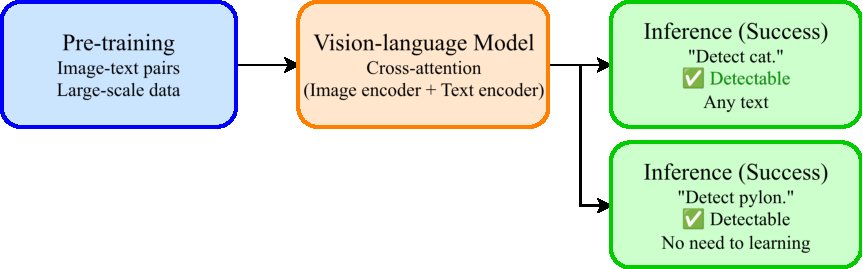
\includegraphics[width=1.0\linewidth]{images/pdf/zero-shot_object_detection.pdf}
\caption{Zero-shot object detection.}
\label{fig:zeroshot_detection}
\end{figure}

% ------------------------------------------------

\newpage

\section{セグメンテーション}
セグメンテーションとは，画像内の各ピクセルに対して所属する物体または領域を識別する技術である．物体検出が矩形領域で物体を捉えるのに対し，セグメンテーションはピクセル単位の精密な領域分割を行う．

\subsection{従来のセグメンテーションとその課題}
セグメンテーションには，画像全体を意味的なクラスに分割するセマンティックセグメンテーションと，個々の物体インスタンスを区別するインスタンスセグメンテーションがある．従来手法であるFCN\cite{fcn}，U-Net\cite{unet}，Mask R-CNN\cite{mask_rcnn}などは，医療画像解析や自動運転などの分野で高精度な結果を達成してきた．

しかし，物体検出と同様に，従来のセグメンテーション手法も固定カテゴリに制約される．学習データに含まれないカテゴリに対しては対応できず，新しいカテゴリを追加するには大量のピクセルレベルのアノテーションが必要となる（\Fig{fig:annotation}）．ピクセル単位のラベル付けは矩形のBBoxよりもはるかに時間とコストがかかるため，この制約はより深刻な問題となる．

\vspace{1cm}

\begin{figure}[H]
\centering
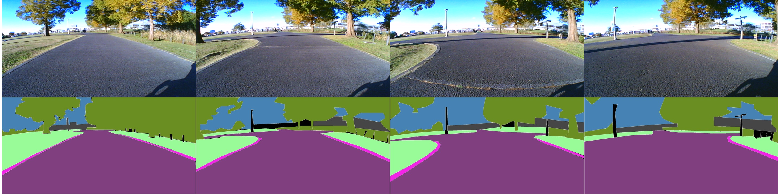
\includegraphics[width=1.0\linewidth]{images/pdf/annotation.pdf}
\caption{Example of creating a dataset for semantic segmentation.}
\label{fig:annotation}
\end{figure}

\newpage

\subsection{ゼロショットセグメンテーション}
ゼロショットセグメンテーションは，学習時に見たことのない物体に対しても，プロンプトに基づいて高精度なマスクを生成する技術である．この技術により，点や矩形などの簡単なプロンプトから，任意の物体のセグメンテーションマスクを得ることが可能となる．

ゼロショットセグメンテーションの実現には，プロンプタブルセグメンテーションという概念が重要である．これは，ユーザーが提供する様々な形式のプロンプト（点，BBoxなど）を入力として受け取り，それに対応するセグメンテーションマスクを生成する技術である．異なる形式のプロンプトを統一的な表現に変換し，画像特徴と融合することで，柔軟なセグメンテーションを実現する(\Fig{fig:promptable_seg_model})．

\vspace{1cm}

\begin{figure}[H]
\centering
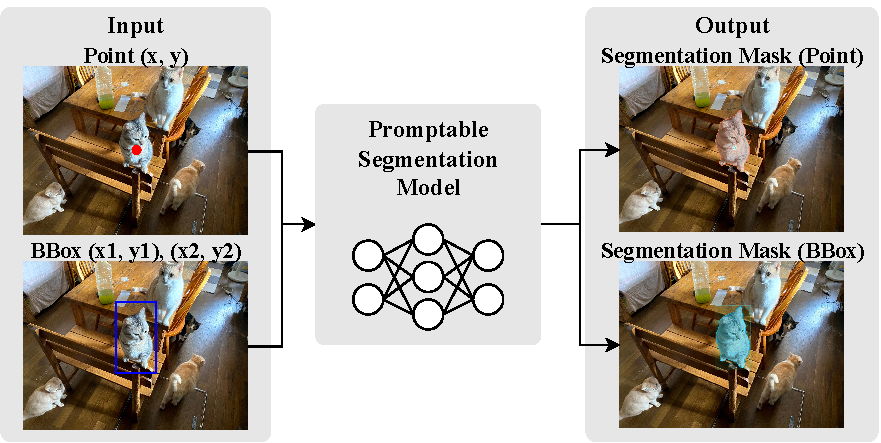
\includegraphics[width=1.0\linewidth]{images/pdf/promptable_seg_model.pdf}
\caption{Prompted zero-shot segmentation.}
\label{fig:promptable_seg_model}
\end{figure}

\newpage

実用的なアプローチとして，ゼロショット物体検出とプロンプタブルセグメンテーションを統合する方法がある(\Fig{fig:text_promptable_seg_model})．まず，テキストプロンプトから物体の位置を検出し，その検出結果をセグメンテーションのプロンプトとして利用する．この2段階の処理により，テキストのみから任意の物体の精密なセグメンテーションが可能となる．従来手法では不可能だった，未知の物体カテゴリに対する対応が実現される．

\vspace{1cm}

\begin{figure}[H]
\centering
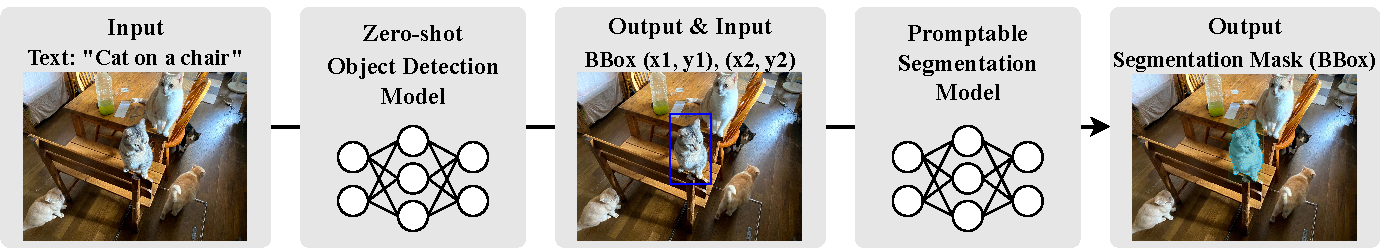
\includegraphics[width=1.0\linewidth]{images/pdf/text_promptable_seg_model.pdf}
\caption{Prompted zero-shot segmentation.}
\label{fig:text_promptable_seg_model}
\end{figure}

\newpage

\section{物体追跡}
物体追跡は，動画内で特定の物体を連続的に識別し，その位置を追跡する技術である．物体検出とセグメンテーションが各フレームで独立に物体を認識するのに対し，物体追跡は時間的な連続性を利用して物体の動きを捉える．この技術は，自動運転における歩行者追跡，スポーツ映像解析，監視システムなど，幅広い応用分野で重要な役割を果たしている．物体追跡手法は主に，疎なオプティカルフローと密なオプティカルフローの2つのアプローチに分類される．

\subsection{疎なオプティカルフロー}
疎なオプティカルフローは，動画内の顕著な特徴点を抽出し，それらの動きを追跡する手法である．代表的な実装であるKLTトラッカー（Kanade-Lucas-Tomasi Feature Tracker）は，以下の手順で動作する．

まず，Shi-Tomasi法\cite{shi_tomasi}により画像内のコーナー特徴点を検出する．この手法は，各ピクセルにおける輝度勾配の固有値を評価し，追跡に適した顕著な特徴点を選択する．次に，検出された特徴点に対してLucas-Kanade法\cite{lucas_kanade}に基づくオプティカルフローを適用する．Lucas-Kanade法は，画像の輝度変化が小さいという仮定のもと，最小二乗法により特徴点の移動ベクトルを計算する．さらに，ピラミッドオプティカルフローを用いることで，異なる解像度の画像階層を利用し，大きな動きにも対応可能となる．

疎なオプティカルフローの主な利点は，計算コストが低く，リアルタイム処理に適している点である．一方で，特徴点が存在しない領域や，テクスチャの乏しい物体に対しては追跡が困難という制約がある．

\newpage

\subsection{密なオプティカルフロー}
密なオプティカルフローは，画像全体のピクセル単位で動きベクトルを推定する手法である．代表的な手法としてHorn-Schunck法\cite{horn_schunck}があり，画像の輝度勾配に基づき全ピクセルの動きを同時に推定する．この手法は，フローの滑らかさの制約を導入することで，ノイズに強い動き推定を実現している．

より高精度な手法として，Farneback法\cite{farneback}やTVL1オプティカルフロー\cite{tvl1}なども広く利用されている．これらの手法は，背景の動きや物体の大規模な変形を捉えるのに適しており，動画の手ぶれ補正や物体の動き解析などに応用される．一方で，全ピクセルの動きを推定するため計算コストが高く，リアルタイム処理には工夫が必要という欠点がある．